\documentclass[11pt]{article}
\usepackage{amsmath,amssymb}
\usepackage{bm}
\usepackage{xcolor}
\usepackage{ctex}
\usepackage{CJK}
\usepackage{float}
\usepackage{amsthm}
\usepackage{geometry}
\geometry{left=2.0cm,right=2.0cm,top=2.5cm,bottom=2.5cm}
\usepackage{algorithmic}
\usepackage{algorithm}           
\newtheorem{myDef}{Definition}[subsection]
\newtheorem{myTheo}{定理}[subsection]
\newtheorem{mylem}{Lemma}[subsection]
\newtheorem{mycor}{推论}[subsection]
\newtheorem{myproof}{证明}[subsection]


\usepackage{geometry} 
\usepackage{indentfirst}
\usepackage{amsthm}
\usepackage{amsmath}
\usepackage{amssymb}
\usepackage{setspace}
\usepackage{geometry}
\usepackage{algorithm}
\usepackage{algorithmic}
\usepackage{multirow}
\usepackage{blkarray}
\usepackage{tikz}

%%%
\newtheorem{theorem}{定理}[subsection]
\floatname{algorithm}{算法}


\usepackage{geometry}      
\geometry{left=2.5cm,right=2.5cm,top=3cm,bottom=3.5cm}    
\usepackage{indentfirst}
\usepackage{CJK}
\usepackage{amsthm}
\usepackage{amsmath}
\usepackage{amssymb}
\usepackage{graphicx}
\usepackage{listings}
\usepackage{setspace}
\usepackage{geometry}
\usepackage{multirow}
\usepackage{xcolor}
\usepackage{cite}
\usepackage{fancyhdr}
\usepackage{ctex}
\usepackage{blkarray}


\newtheorem{lemma}{引理}[subsection]
\newtheorem{inference}{推论}[subsection]

\lstset{ 
    basicstyle=\tt,
    rulesepcolor=\color{red!20!green!20!blue!20},
    escapeinside=``,
    xleftmargin=2em,xrightmargin=2em, aboveskip=1em,
    framexleftmargin=1.5mm,
    frame=shadowbox,
    backgroundcolor=\color[RGB]{245,245,244},
    keywordstyle=\color{blue}\bfseries,
    identifierstyle=\bf,
    numberstyle=\color[RGB]{0,192,192},
    commentstyle=\it\color[RGB]{96,96,96},
    stringstyle=\rmfamily\slshape\color[RGB]{128,0,0},
    showstringspaces=false
}



\lstdefinestyle{C}{
 language={[ANSI]C},
 numbers=left,
 numberstyle=\tiny,
 basicstyle=\small\ttfamily,
 stringstyle=\color{purple},
 keywordstyle=\color{blue}\bfseries,
 commentstyle=\color{olive},
 directivestyle=\color{blue},
 frame=shadowbox,
 %framerule=0pt,
 %backgroundcolor=\color{pink},
 rulesepcolor=\color{red!20!green!20!blue!20}
 %rulesepcolor=\color{brown}
 %xleftmargin=2em,xrightmargin=2em,aboveskip=1em
}


\pagestyle{fancy}





% Edit these as appropriate
\newcommand\course{差分方法\uppercase\expandafter{\romannumeral2}}
\newcommand\hwnumber{}                  % <-- homework number
\newcommand\name{陈伟}                 % <-- Name
\newcommand\ID{1901110037}           % <-- ID

\pagestyle{fancyplain}
\headheight 35pt
\lhead{\name\\\ID}                 
\chead{\textbf{\Large  差分方法\uppercase\expandafter{\romannumeral2} lab2\hwnumber}}
\rhead{\course \\ \today}
\lfoot{}
\cfoot{}
\rfoot{\small\thepage}
\headsep 1.5em




\title{差分方法\uppercase\expandafter{\romannumeral2}\\
lab2\\
Oliker-Prussner method 算例\\
陈伟\\
1901110037}

\begin{document}

\maketitle % —— 显示标题
\tableofcontents %—— 制作目录(目录是根据标题自动生成的)

\newpage
\section{问题描述}
用 Oliker-Prussner method 求解2D的Monge-Ampère方程:
$$\left\{\begin{aligned}
\operatorname{det} D^{2} u &=f \quad \text { in } \Omega \subset \mathbb{R}^{2} \\
u &=g \quad \text { on } \partial \Omega
\end{aligned}\right.$$
其中计算区域为$\Omega=(-1,1)^2.$令$\bm{x}=(x,y)^T$. 对于如下三个例子进行数值实验:
\begin{itemize}
\item Smooth and radial example:
$$u(\bm{x})=\text{exp}(\vert{\bm{x}}\vert^2/2),\quad f(\bm{x})=(1+\vert{\bm{x}})\vert^2\text{exp}(\vert{\bm{x}}\vert^2).$$
\item Piecewise smooth solution:
$$\begin{array}{lll}
u(\boldsymbol{x}) & =\left\{\begin{array}{ll}
2|\boldsymbol{x}|^{2} & |\boldsymbol{x}| \leq 1 / 2, \\
2(|\boldsymbol{x}|-1 / 2)^{2}+2|\boldsymbol{x}|^{2} & |\boldsymbol{x}| \geq 1 / 2
\end{array}\right. \\
f(\boldsymbol{x}) & =\left\{\begin{array}{ll}
16 & |\boldsymbol{x}| \leq 1 / 2 \\
64-16|\boldsymbol{x}|^{-1} & |\boldsymbol{x}| \geq 1 / 2
\end{array}\right.
\end{array}$$
\item Singular solution $u\in W_p^2$ with $p < 2:$:
$$\begin{array}{lll}
u(\boldsymbol{x}) & =\left\{\begin{array}{ll}
x^{4}+\frac{3}{2} x^{-2} y^{2} & |y| \leq|x|^{3} \\
\frac{1}{2} x^{2} y^{2 / 3}+2 y^{4 / 3} & |y|>|x|^{3}
\end{array}\right. \\
f(\boldsymbol{x}) & =\left\{\begin{array}{ll}
36-9 x^{-6} y^{2} & |y| \leq|x|^{3} \\
\frac{8}{9}-\frac{5}{9} x^{2} y^{-2 / 3} & |y|>|x|^{3}
\end{array}\right.
\end{array}$$
\end{itemize}
边界$g(\bm{x})$可以通过真解获得. 报告并且讨论:

\begin{itemize}
\item The convergence history of the discrete Perron iteration;
\item Errors in $L^\infty{}$ and convergence order w.r.t. the mesh sizes;
\item Errors and convergence order in the discrete $W_p^2$ norms. Here, the discrete $W_p^2$ norm is defined by
$$\|v\|_{W_{p}^{2}\left(\mathcal{N}_{h}^{I}\right)}^{p}=\sum_{j=1}^{4} \sum_{x_{i} \in \mathcal{N}_{h}^{I}}\left|\omega_{i}\right| \cdot\left|\Delta_{e_{j}} v\left(x_{i}\right)\right|^{p}$$
\end{itemize}
其中$e_1=(1,0),\ e_2=(0,1),\ e_3=(1,1),\ $与$e_4=(1,-1)$和
$$\Delta_{e} v\left(x_{i}\right):=\frac{v\left(x_{i}+h e\right)-2 v\left(x_{i}\right)+v\left(x_{i}-h e\right)}{\left|e^{2}\right| h^{2}}$$
$\omega_{i}$表示以$x_i$为心的单元集合.
\section{求解方法}
\subsection{Oliker-Prussner method}
目标:对于给定的节点集合$N_h=N_h^0\cup N_h^\partial$,且$N_h^0$是translation invariant的,找凸的点值函数$u_h$,使得
$$\vert{\partial u_h(x_i)}\vert=f_i, \forall x_i\in N_h^0$$
其中$f_i=\int_{\Omega_i}f(x)\phi_i(x)dx , \partial x_i\in N_h^0$,
$\phi_i(x)$是$x_i$点的基函数。

\begin{algorithm}[H]
%\label{G_theta}
\caption{Oliker-Prussner method} 
\begin{algorithmic}[]
\setstretch{1.2}
\STATE STEP1: Initialization. 取$\Lambda,R$充分大,考虑$p(x)=\frac{\Lambda^{1/d}}{2}(\vert{x}\vert^2-2R^2)$, 令$u_h^0=N_hp$, $\Gamma{}_h^0$为$N_h$下的Delaunay triangulation.
上述$\Lambda, R$应满足
$$\begin{aligned}
\vert{\partial u_h^0(x_i)}\vert&\geqslant f_i,\forall x_i\in N_h^0\\
u_h^0&\leqslant I_h^0g\ on\ \partial\Omega_h
\end{aligned}$$

\STATE STEP2:  对于边界点循环,令$u_h^0(x_i)=g(x_i),$  同时更新网格使得$\Gamma{}_h^0$是凸的,对于能Flip的边,直接Flip, 不能Flip的边,只能是平四边形,提升还未提升的边界点$x_k$为$g(x_k)$即可.

\STATE STEP3: 提升内部网格点$x_i$的值,如果$u_h^k$已经计算好了,而且对于$j<i,$的$u^{k+1}_h(x_j)$也计算好了,提升$u_h^{k+1}(x_i),$使得
$$\vert{\partial u_h^{k+1}(x_i)}\vert=f_i$$
注意提升$x_i$的值的时候,可能会引起网格变动,我们需要变动网格$\Gamma{}^{k+1}_h$,使得其网格函数$\Gamma{}^{k+1}_h(u^{k+1}_h)$仍是凸函数,但是总能提升$u_h^{k+1}(x_i)$
使得上式成立。关于提升方法我们后面提

\STATE STEP4: 循环STEP3直到
$$\max_{x_i\in N_h^0}(\vert{\partial u_h^{k+1}(x_i)}\vert-f_i)< \text{Tol}$$
其中Tol为某个可允许误差.
\end{algorithmic}
\end{algorithm}

\subsection{提升$u_h^{k}(x_i)$方法}
考虑$x_i$为如下中心点$o$

\begin{figure}[H]
\begin{center}
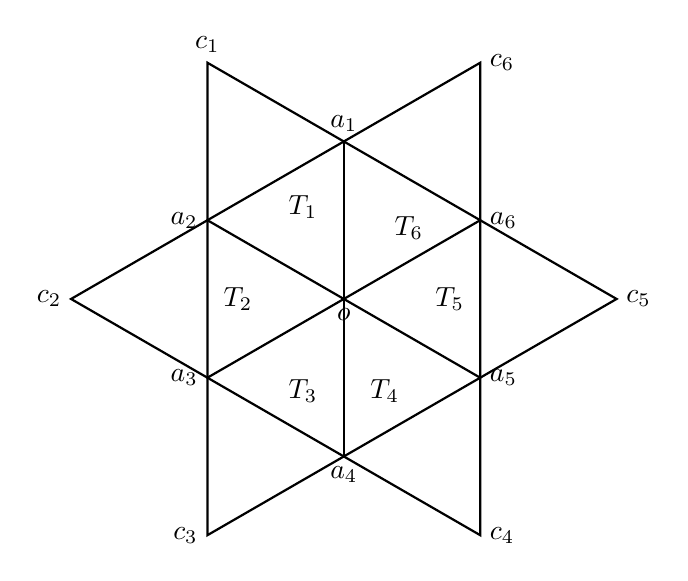
\begin{tikzpicture}
 \coordinate (o) at (0,0);
 \coordinate (a1) at (0,2);
 \coordinate (a6) at (1.7321,1.0);
 \coordinate (a5) at (1.7321,-1.0);
 \coordinate (a4) at  (0,-2.0);
 \coordinate (a3) at (-1.7321,-1.0);
 \coordinate (a2) at  (-1.7321,1.0);


\coordinate (a12) at ( -1.7321 ,   3.0000);
\coordinate (a23) at  (-3.4641  ,  0.0000);
\coordinate (a34) at   ( -1.7321,   -3.0000);
\coordinate (a45) at   (1.7321 ,  -3.0000);
\coordinate (a56) at   ( 3.4641 ,   0.0000);
\coordinate (a61) at   ( 1.7321  ,  3.0000);

\coordinate (T6) at (0.5196  , 0.9000);
\coordinate (T5) at (1.0392  ,  0.0000);
\coordinate (T4) at ( 0.5196  , -0.9000);
\coordinate (T3) at ( -0.5196 ,  -0.9000);
\coordinate (T2) at (-1.0392  ,  0.0000);
\coordinate (T1) at (-0.5196  ,   0.9000);


\draw[thick] (o)--(a1);
\draw[thick] (o)--(a2);
\draw[thick] (o)--(a3);
\draw[thick] (o)--(a4);
\draw[thick] (o)--(a5);
\draw[thick] (o)--(a6);
\draw[thick] (a1)--(a2)--(a3)--(a4)--(a5)--(a6)--(a1);

\draw[thick] (a1)--(a12)--(a2)--(a23)--(a3)--(a34)--(a4)--(a45)--(a5)--(a56)--(a6)--(a61)--(a1);


\node [below] at (o) {$o$};
\node [above] at (a1) {$a_1$};
\node [left] at (a2) {$a_2$};
\node [left] at (a3) {$a_3$};
\node [below] at (a4) {$a_4$};
\node [right] at (a5) {$a_5$};
\node [right] at (a6) {$a_6$};

\node [above] at (a12) {$c_1$};
\node [left] at (a23) {$c_2$};
\node [left] at (a34) {$c_3$};
\node [right] at (a45) {$c_4$};
\node [right] at (a56) {$c_5$};
\node [right] at (a61) {$c_6$};

\node [above] at (T1) {$T_1$};
\node [left] at (T2) {$T_2$};
\node [below] at (T3) {$T_3$};
\node [below] at (T4) {$T_4$};
\node [right] at (T5) {$T_5$};
\node [right] at (T6) {$T_6$};




\end{tikzpicture}
\end{center}
\end{figure}

如果原来网格函数是凸的,则我们提升 $o$点值后, 可能会jump小于0的边是$oa_1,oa_2,oa_3,\cdots{},oa_6$, 同时,我们也可以算出这些边jump为0时的$u_h^{k}(x_i)$需要提升的值,分别记作$\theta_1,\theta_2,\cdots{},\theta_6$. 不妨设其中最小的一个为$\theta_1,$对应的边也即是$oa_1$, 我们先在$[u_h^{k}(x_i),u_h^{k}(x_i)+\theta_1]$中找是否有使得
$\vert{\partial u_h^{k+1}(x_i)}\vert=f_i$
成立的$u_h^{k+1}(x_i)$, 为此我们要计算梯度凸包的面积,为此我们先考虑如下相邻情况的梯度面积

\begin{figure}[H]
\begin{center}
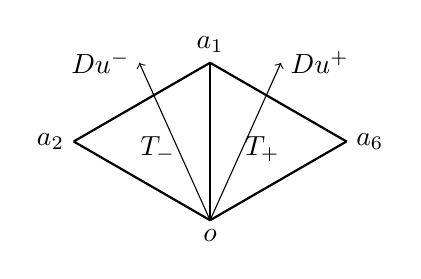
\begin{tikzpicture}
 \coordinate (o) at (0,0);
 \coordinate (a1) at (0,2);
 \coordinate (a6) at (1.7321,1.0);
 \coordinate (a2) at  (-1.7321,1.0);



\coordinate (T6) at (0.3196  , 0.9000);
\coordinate (T1) at (-0.3196  ,   0.9000);

\coordinate (DTp) at (0.9  , 2.000);
\coordinate (DTn) at (-0.9  , 2.000);

\draw[thick] (o)--(a1);
\draw[thick] (o)--(a2);
\draw[thick] (o)--(a6);
\draw[thick] (a1)--(a2);
\draw[thick] (a6)--(a1);

\draw[->] (o)--(DTp);
\draw[->] (o)--(DTn);

\node [below] at (o) {$o$};
\node [above] at (a1) {$a_1$};
\node [left] at (a2) {$a_2$};
\node [right] at (a6) {$a_6$};



\node [left] at (T1) {$T_-$};
\node [right] at (T6) {$T_+$};
\node [right] at (DTp) {$Du^+$};
\node [left] at (DTn) {$Du^-$};

\end{tikzpicture}
\end{center}
\end{figure}

假设我们$a_1,a_6,a_2$处的值已经给好,并且
$$\begin{aligned}
\widehat{Du}^+&=u_h(a_6)D\lambda_6+u_h(a_1)D\lambda_1|_{T_+}\\
\widehat{Du}^-&=u_h(a_2)D\lambda_2+u_h(a_1)D\lambda_1|_{T_-}
\end{aligned}$$
已经计算出,这样我们有
$$\begin{aligned}
Du^+ &= \widehat{Du}^++u_h(o)D\lambda_o|_{T_+}\\
Du^-&=\widehat{Du}^-+u_h(o)D\lambda_o|_{T_-}
\end{aligned}$$
这样我们的这两个梯度形成的面积就是
$$\begin{aligned}
S|_{oa_1}&=Du^+\times Du^-\\
&= u_h(o)^2 \left(D\lambda_o|_{T^+}\times D\lambda _o|_{T^-}\right)\\
&+u_h(o)\left(\widehat{Du}^+\times D\lambda_o|_{T_-}+D\lambda_o|_{T_+}\times \widehat{Du}^-\right)+ (\widehat{Du}^+\times \widehat{Du}^-)\\
&= A_{oa_1}u_h(o)^2+B_{oa_1}u_h(o)+C_{oa_1}
\end{aligned}$$
同样的方式我们把其它边上的两个相邻单元的梯度形成的三角形面积算出来,再加起来就有
$$S(u_h(o)) = Au_h(o)^2+Bu_h(o)+C$$
%注意由次梯度面积随着$u_h^{k}(x_i)$的提升是单调减小的,所以我们可以先计算$S()$
也就是一个二次函数,下面我们求解方程:
$$S(x)=f_i$$若存在$x^*\in[u_h^{k}(x_i),u_h^{k}(x_i)+\theta_1]$,这我们提升$u_h^k(x_i)$的值为$x^*$即可,否则我们提升其值为$u_h^{k}(x_i)+\theta_1,$同时将$oa_1$flip, 并重新找$x_i$相关联的单元重复上面的事情。对于有如下平四边形出现时
\begin{figure}[H]
\begin{center}
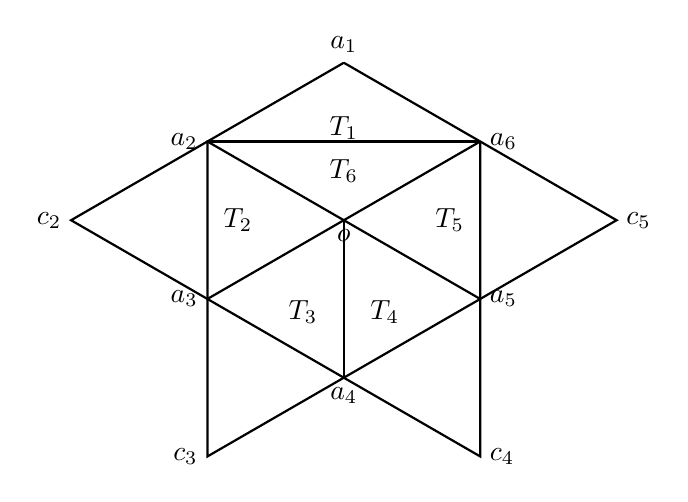
\begin{tikzpicture}
 \coordinate (o) at (0,0);
 \coordinate (a1) at (0,2);
 \coordinate (a6) at (1.7321,1.0);
 \coordinate (a5) at (1.7321,-1.0);
 \coordinate (a4) at  (0,-2.0);
 \coordinate (a3) at (-1.7321,-1.0);
 \coordinate (a2) at  (-1.7321,1.0);


\coordinate (a12) at ( -1.7321 ,   3.0000);
\coordinate (a23) at  (-3.4641  ,  0.0000);
\coordinate (a34) at   ( -1.7321,   -3.0000);
\coordinate (a45) at   (1.7321 ,  -3.0000);
\coordinate (a56) at   ( 3.4641 ,   0.0000);
\coordinate (a61) at   ( 1.7321  ,  3.0000);

\coordinate (T6) at (0.0  , 0.9000);
\coordinate (T5) at (1.0392  ,  0.0000);
\coordinate (T4) at ( 0.5196  , -0.9000);
\coordinate (T3) at ( -0.5196 ,  -0.9000);
\coordinate (T2) at (-1.0392  ,  0.0000);
\coordinate (T1) at (-0.0  ,   0.9000);



\draw[thick] (o)--(a2);
\draw[thick] (o)--(a3);
\draw[thick] (o)--(a4);
\draw[thick] (o)--(a5);
\draw[thick] (o)--(a6);
\draw[thick] (a1)--(a2)--(a3)--(a4)--(a5)--(a6)--(a1);
\draw[thick] (a2)--(a6);

\draw[thick](a2)--(a23)--(a3)--(a34)--(a4)--(a45)--(a5)--(a56)--(a6);%--(a61)--(a1);


\node [below] at (o) {$o$};
\node [above] at (a1) {$a_1$};
\node [left] at (a2) {$a_2$};
\node [left] at (a3) {$a_3$};
\node [below] at (a4) {$a_4$};
\node [right] at (a5) {$a_5$};
\node [right] at (a6) {$a_6$};

%\node [above] at (a12) {$c_1$};
\node [left] at (a23) {$c_2$};
\node [left] at (a34) {$c_3$};
\node [right] at (a45) {$c_4$};
\node [right] at (a56) {$c_5$};
%\node [right] at (a61) {$c_6$};

\node [above] at (T1) {$T_1$};
\node [left] at (T2) {$T_2$};
\node [below] at (T3) {$T_3$};
\node [below] at (T4) {$T_4$};
\node [right] at (T5) {$T_5$};
\node [below] at (T6) {$T_6$};




\end{tikzpicture}
\end{center}
\end{figure}
其中$T_2T_6,$于$T_5T_6$形成的四边形都是平四边形,这也意味着$oa_2$与$oa_6$都不能被flip. 若$a_2,a_3,a_6,o$连同它们对应的值在三维空间中共面,也即是$oa_2$的jump为0了,这样我们不妨记在$T_2,T_6$上的梯度为$Du,$在$T_3,T_3,T_5$上的梯度为$Du_3,Du_4,Du_5,$ 由连续性有$Du_3,Du_5$在$a_3a_6$上的分量都与$Du$在$a_3a_6$上的分量相同, 这样$Du_3-Du_5$是与$a_3a_6$垂直的, 同时
$$Du_3-Du_5=Du_3-Du_4+Du_4-Du_5$$
等式右端前者是垂直$oa_4$指向$a_3$的,后者是垂直$oa_5$指向$a_4$的,这样两者正方向的线性组合得到的向方向不可能与$a_3a_6$的垂直方向相同,除非$Du_3=Du_4=Du_5$,这也意味着这种情况下的次梯度面积为0. 对于凹四边形也同理。 这样当我们的$f_i$大于0时,我们一定不会flip平四边形或凹四边形的情况!





\section{数值算例}

对三个例子取Tol=1e-5, 正规网格剖分,取$h =1, 1/2,1/4,1/8,1/16$,得到的结果如下
,其中图片Perron iteration过程横坐标是迭代次数,纵坐标是的err是
$$\text{err}= \max_{x_i\in N_h^0}\vert{\partial u^k_h(x_i)}\vert-f_i$$

\subsection{example1 $u\in C^\infty{}(\bar{\Omega})$光滑算例}
取$\Lambda=25,R = 1.5,$ 得到的结果如下
\begin{table}[ht!]
\centering
\caption{example1 光滑算例结果}
\label{table}
    \begin{tabular}{  c| c|c c|c c| c c }
          \hline      
  \hline
  
\hline



    \hline     
  
  
\hline



    \hline     
    \hline   
    
 h  &迭代次数  	&$L^\infty{}$& rate&$W_1^2$&rate&$W_2^2$&rate\\

1&1&8.10e-02	&0.00	&9.72e-01	&0.00	&3.62e-01	&0.00\\
1/2&24&2.59e-02	&1.64	&1.33e+00	&-0.46	&3.12e-01	&0.21\\
1/4&89&7.04e-03	&1.88	&6.31e-01	&1.08	&1.43e-01	&1.12\\
1/8&324&1.87e-03	&1.91	&2.15e-01	&1.55	&4.81e-02	&1.58\\
1/16&1170&8.82e-04	&1.08	&8.06e-02	&1.42	&1.53e-02	&1.66\\
      \hline      
  \hline
  
\hline



    \hline     
    \hline
 
  \hline
  
\hline


    \end{tabular}
\end{table}




\begin{figure}[htp!]
\centering
\caption{example1 算例Perron iteration过程}
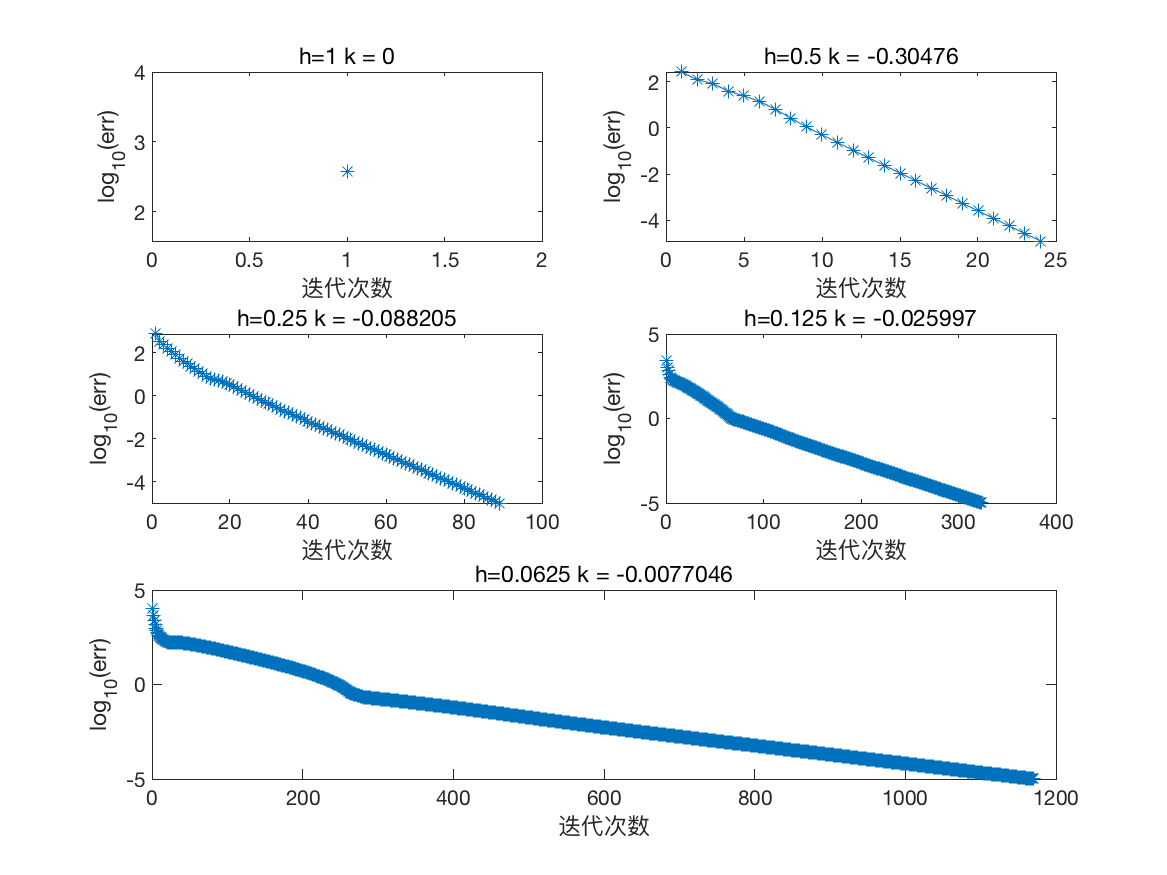
\includegraphics[width=0.5\textwidth]{1.png}
\end{figure}


\clearpage


\subsection{example2 $u\in W_\infty^2$分片光滑算例}
取$\Lambda=100,R=1.5$, 得到的结果如下
\begin{table}[ht!]
\centering
\caption{example2 分片光滑算例结果}
\label{table}
    \begin{tabular}{  c| c|c c|c c| c c }
          \hline      
  \hline
  
\hline



    \hline     
  
  
\hline



    \hline     
    \hline   
    
 h  &迭代次数  	&$L^\infty{}$& rate&$W_1^2$&rate&$W_2^2$&rate\\

1&1&2.07e-01	&0.00	&4.34e+00	&0.00	&1.22e+00	&0.00\\
1/2&26&3.50e-02	&2.56	&3.04e+00	&0.51	&6.98e-01	&0.81\\
1/4&100&1.47e-02	&1.25	&1.61e+00	&0.92	&4.05e-01	&0.79\\
1/8&368&4.93e-03	&1.58	&9.04e-01	&0.83	&3.10e-01	&0.38\\
1/16&1343&9.34e-04	&2.40	&1.45e-01	&2.64	&3.49e-02	&3.15\\
      \hline      
  \hline
  
\hline



    \hline     
    \hline
 
  \hline
  
\hline


    \end{tabular}
\end{table}





\begin{figure}[htp!]
\centering
\caption{example2 算例Perron iteration过程}
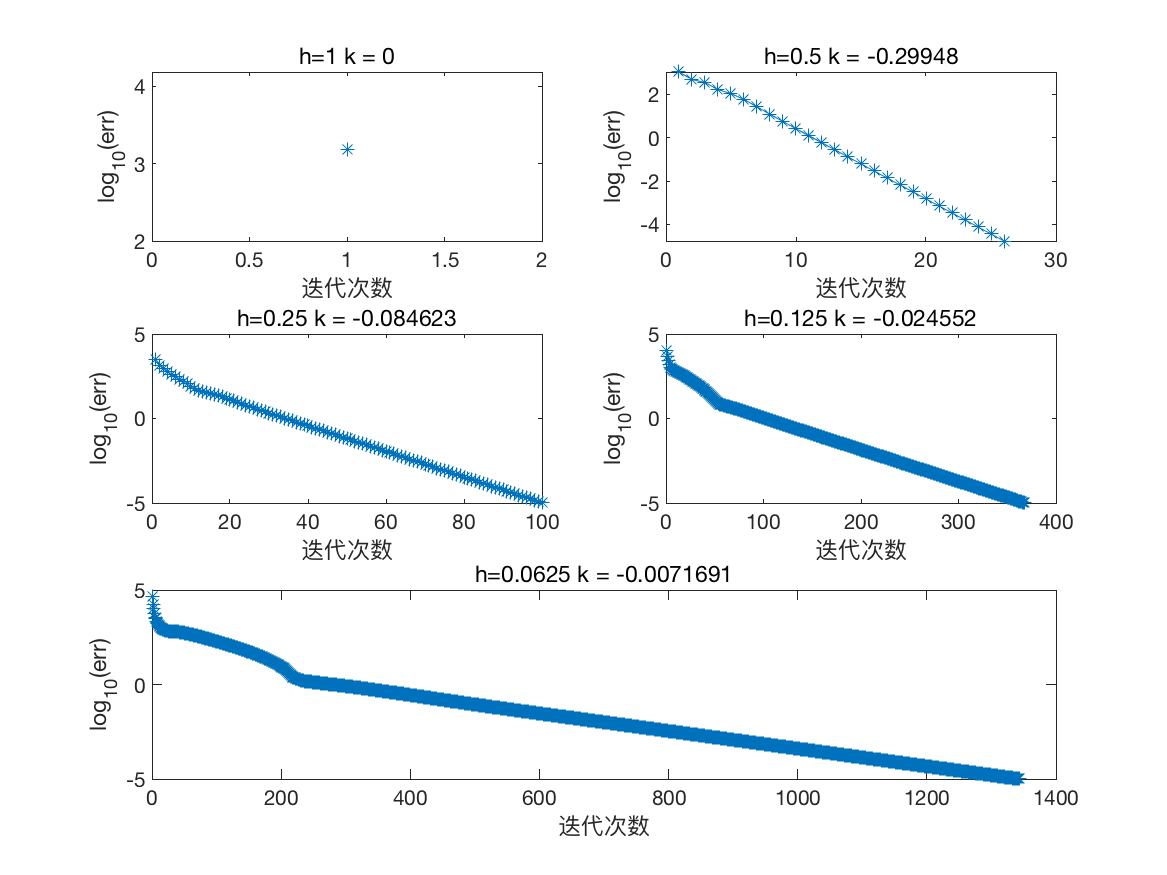
\includegraphics[width=1.0\textwidth]{2.png}
\end{figure}







\subsection{example3 $u\in W^2_p, p<2$ 含有奇点算例}

取$\Lambda=100,R=1.5$,得到的结果如下

\begin{table}[!htbp]
\centering
\caption{example3 含有奇点算例结果}
\label{table}
    \begin{tabular}{  c| c|c c|c c| c c }
          \hline      
  \hline
  
\hline



    \hline     
  
  
\hline



    \hline     
    \hline   
    
 h  &迭代次数  	&$L^\infty{}$& rate&$W_1^2$&rate&$W_2^2$&rate\\

1&1&2.23e-01	&0.00	&5.36e+00	&0.00	&1.41e+00	&0.00\\
1/2&27&1.31e-01	&0.77	&1.24e+01	&-1.21	&2.97e+00	&-1.07\\
1/4&109&4.74e-02	&1.46	&1.15e+01	&0.11	&2.80e+00	&0.09\\
01/8&408&1.56e-02	&1.61	&7.96e+00	&0.54	&2.42e+00	&0.21\\
1/16&1531&7.42e-03	&1.07	&5.08e+00	&0.65	&2.10e+00	&0.20\\ 


      \hline      
  \hline
  
\hline



    \hline     
    \hline
 
  \hline
  
\hline


    \end{tabular}
\end{table}

\begin{figure}[htp!]
\centering
\caption{example3 算例Perron iteration过程}
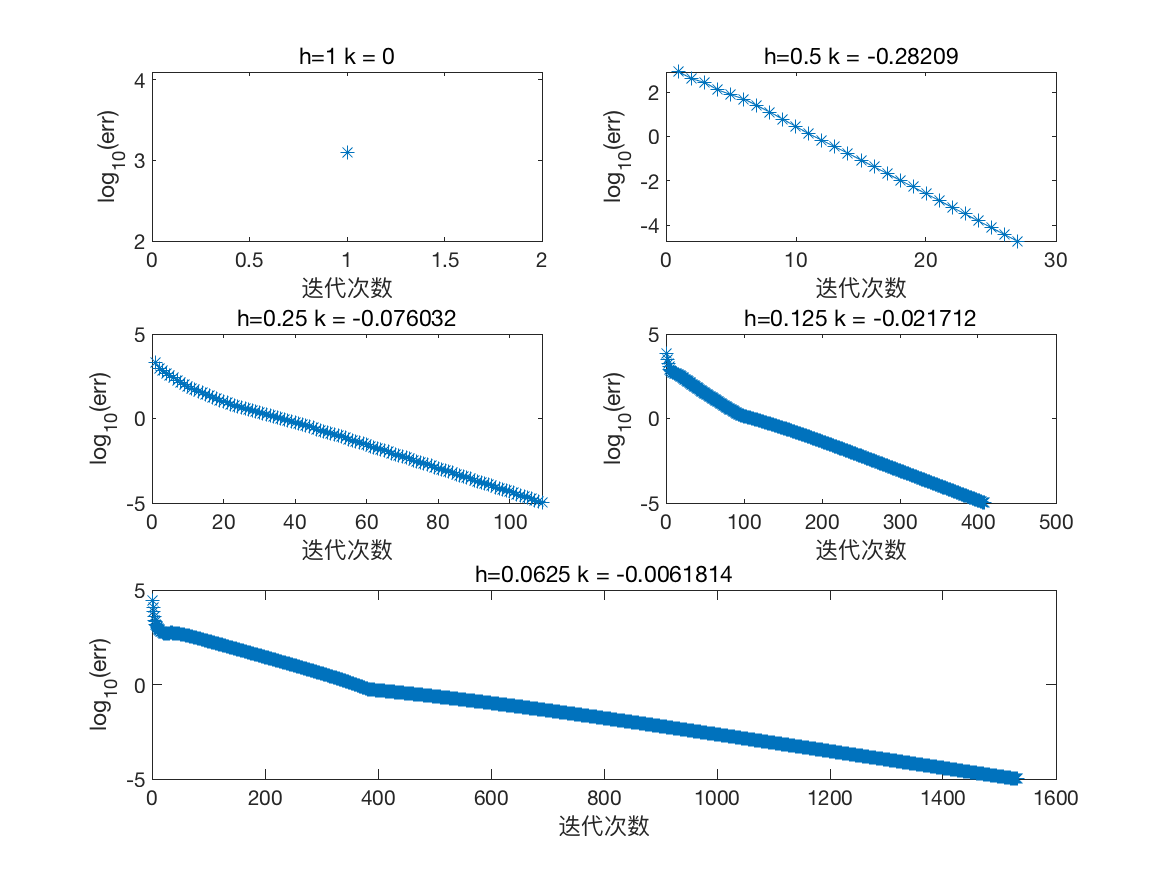
\includegraphics[width=1.0\textwidth]{3.png}
\end{figure}


\clearpage

\section{结果分析}
\subsection{误差收敛阶}
从我们的数值结果来看,对于光滑例子example1的$L^\infty{}$误差,我们大概有二阶收敛性, 其$W_1^2,W_2^2$误差大概有1.5阶左右的样子。对于分片光滑例子example2,其$L^\infty{}$误差结果不太清晰,但大概还是有1.5阶左右的样子,其$W_1^2,W_2^2$大概在1阶左右的样子。对于含有奇点的例子example3,其$L^\infty{}$误差大概在1.5阶左右,其$W_1^2$大概是0.5阶,其$W_2^2$大概在0.2阶的样子.




\subsection{Perron iteration过程收敛速度}

三个算例中Perron iteration过程是相似的,可以看出$\log_{10}(err)$关于迭代次数大致是线性下降的, 而对于其下降斜率$-k,$大致又和$h^2$是线性关系的,我们用线性函数来拟合,得到的结果为
\begin{figure}[htp!]
\centering
\caption{Perron iteration过程下降斜率$-k$与$h$的关系}
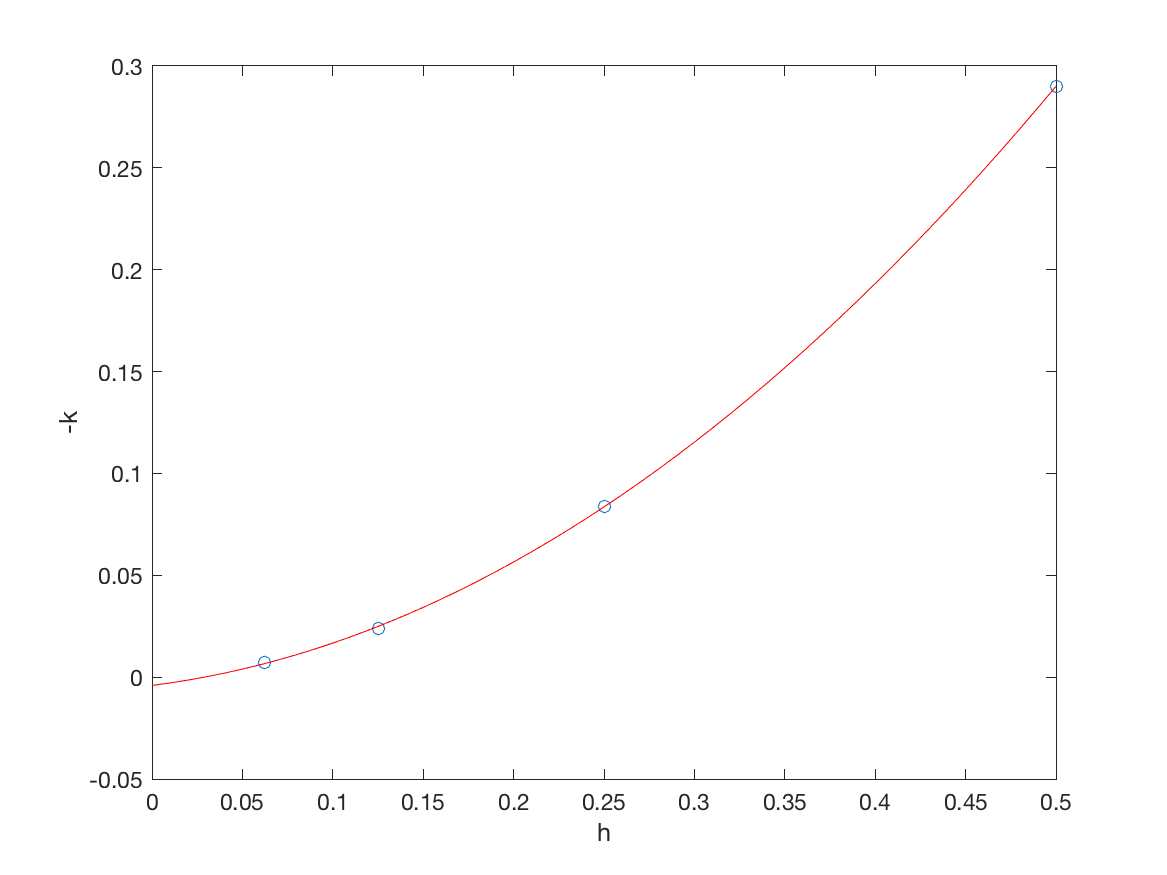
\includegraphics[width=0.8\textwidth]{4.png}
\end{figure}
对应的二次函数为
$$k=-(0.9511h^2+0.1127h-0.0041)=-p(h)$$
这样我们有:
$$\frac{err(i+1)}{err(i)}=10^{k}=10^{-p(h)}$$

\section{代码说明}
本次程序使用matlab编写,包含main.m和Readme.txt等在内一共有20个文件,在文件夹‘matlabcode’中. 关于各文件的含义以及main.m的运行参见Readme.txt.





\end{document}